\documentclass{article}

\usepackage{graphicx}
\usepackage{tikz}
\usepackage{tikzsymbols}
\usetikzlibrary{calc,patterns,shapes.geometric}
\pagestyle{empty}
\usepackage[margin=0pt]{geometry}
\geometry{papersize={14in,12in}}

\def\centerarc[#1](#2)(#3:#4:#5){\draw[#1] ($(#2)+({#5*cos(#3)},{#5*sin(#3)})$) arc (#3:#4:#5);}

\begin{document}
	\begin{figure}
		\centering
		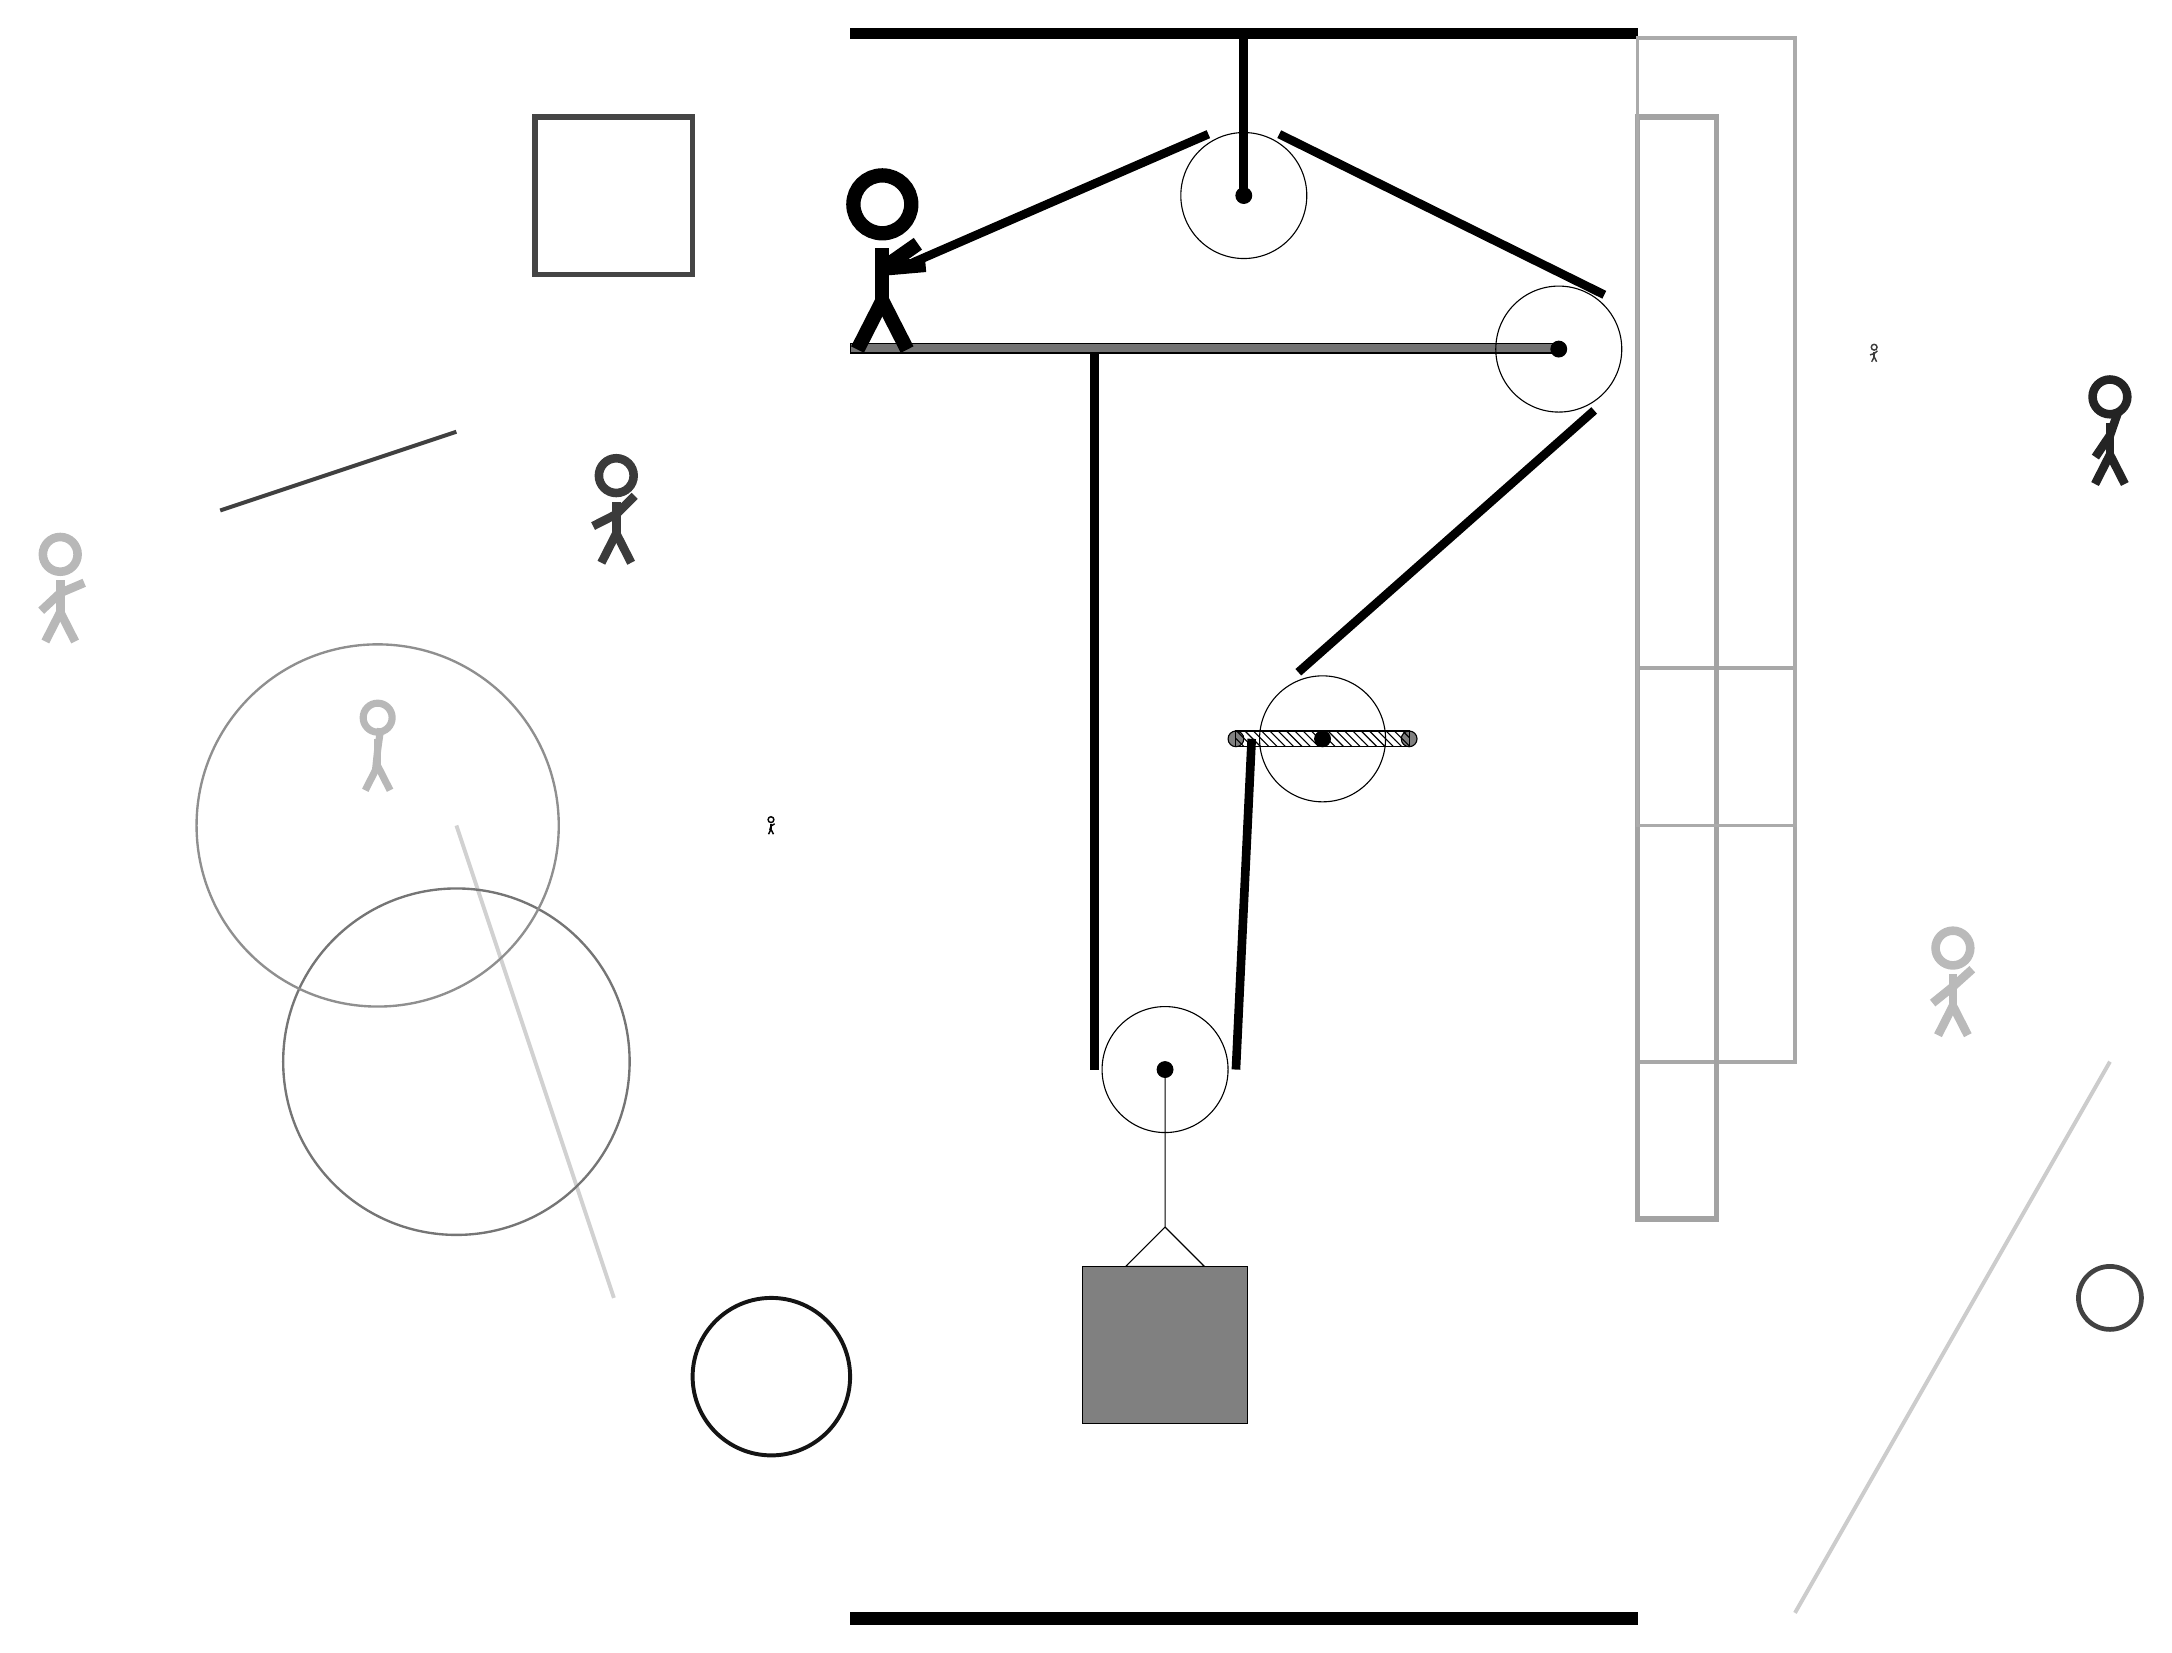
\begin{tikzpicture}
			%%%%% START %%%%%
			
			\draw[fill=black] (-2, 18) rectangle (8, 18.125);
			
			\draw[fill=black!55] (-2, 14) rectangle (7, 14.125);
			
			\draw (2, 4.9) circle (0.8);
			\draw[fill=black] (2, 4.9) circle (0.1);
			
			\draw (7, 14.05) circle (0.8);
			\draw[fill=black] (7, 14.05) circle (0.1);
			
			\draw[fill=white](4, 9.1) circle (0.8);
			\draw[fill=black] (4, 9.1) circle (0.1);
			\draw[fill=black!50] (2.9, 9.1) circle (0.1);
			\draw[fill=black!50] (5.1, 9.1) circle (0.1);
			\draw[pattern=north west lines, pattern color=black] (2.9, 9.2) rectangle (5.1, 9.0);
			
			\draw (3, 16) circle (0.8);
			\draw[fill=black] (3, 16) circle (0.1);
			\draw[line width=1.1mm] (3, 16) -- (3, 18);
			
			\draw (2, 4.9) -- (2, 2.9) -- (1.5, 2.4) -- (2.5, 2.4) -- (2, 2.9);
			\draw[fill=black!50] (0.95, 2.4) rectangle (3.05, 0.4);
			
			\draw[line width=1.1mm] (1.1, 14) -- (1.1, 4.9);
			\centerarc[line width=1.1mm](2, 4.9)(180:360:0.9);
			\draw[line width=1.1mm](2.9, 4.9) -- (3.1, 9.1);
			\centerarc[line width=1.1mm](4, 9.1)(110:180:0.9);
			\draw[line width=1.1mm](3.6922, 9.9457) -- (7.45, 13.2706);
			\centerarc[line width=1.1mm](7, 14.05)(-60:50:0.9);
			\draw[line width=1.1mm](7.5785, 14.7394) -- (3.45, 16.7794);
			\centerarc[line width=1.1mm](3, 16)(60:120:0.9);
			\draw[line width=1.1mm](2.55, 16.7794) -- (-1.2, 15.15);
			
			\draw[line width=0.5mm, color=black!18](-5, 2) -- (-7, 8);
			
			\draw [line width=0.3mm, color=black!54](-7, 5) circle (2.2);
			\draw[line width=0.7mm, color=black!73] (-4, 15) rectangle (-6, 17);
			\node[line width=0.3mm, color=black!28] at (-12, 11) {\Strichmaxerl[6][43][23]};
			\draw[line width=0.5mm, color=black!34] (10, 10) rectangle (8, 5);
			\node[line width=0.4mm, color=black!27] at (12, 6) {\Strichmaxerl[6][39][42]};
			\node[line width=0.2mm, color=black!77] at (-5, 12) {\Strichmaxerl[6][27][45]};
			
			\draw[line width=0.7mm, color=black!36] (9, 17) rectangle (8, 3);
			\node[line width=0.3mm, color=black!86] at (14, 13) {\Strichmaxerl[6][56][71]};
			
			\node[line width=0.4mm, color=black!28] at (-8, 9) {\Strichmaxerl[5][84][82]};
			\draw [line width=0.3mm, color=black!44](-8, 8) circle (2.3);
			
			\draw[line width=0.5mm, color=black!20](10, -2) -- (14, 5);
			\draw [line width=0.6mm, color=black!74](14, 2) circle (0.4);
			\draw[line width=0.5mm, color=black!75](-7, 13) -- (-10, 12);
			\draw [line width=0.5mm, color=black!92](-3, 1) circle (1.0);
			\node[line width=0.4mm, color=black!76] at (11, 14) {\Strichmaxerl[1][16][41]};
			
			\node[line width=0.2mm, color=black!99] at (-3, 8) {\Strichmaxerl[1][73][32]};
			\draw[line width=0.4mm, color=black!33] (8, 8) rectangle (10, 18);
			
			\node at (-1.5, 15.15) {\Strichmaxerl[10][-175][35]};
			
			\draw[fill=black] (-2, -2) rectangle (8, -2.15);
			
			%%%%% END %%%%%
		\end{tikzpicture}
	\end{figure}	
\end{document}